\section{Apache Hadoop}
\label{sec:hadoop}

\textbf{Apache\texttrademark Hadoop\textregistered}\footnote{\url{https://hadoop.apache.org/}} ist ein Open"=Source"=Software"=Projekt, welches die Verarbeitung von großen Datenmengen auf einem verteilten System ermglicht.
Hadoop wird von der \emph{Apache Foundation} entwickelt und enthält verschiedene vollständig skalierbare Komponenten.
Es ist daher möglich, ein Hadoop"=Cluster auf nur einem einzelnen PC, aber auch verteilt auf ein ganzen Serverzentrum auszuführen.
Hadoop besteht aus folgenden Kernmodulen \cite{HadoopHomePage}:

\begin{description}
	\item[Hadoop Common] Gemeinsam genutzte Kernkomponenten
	\item[Hadoop YARN] Framework zur Verteilung und Ausführung von Anwendungen und das dazugehörige Ressourcen"=Management
	\item[\acl{HDFS}] Kurz \acs{HDFS}, Verteiltes Dateisystem\acused{HDFS}
	\item[Hadoop MapReduce] YARN"=Basiertes System zum Verarbeiten von großen Datenmengen
\end{description}

Hadoop ermöglicht es dadurch, sehr einfach Anwendungen auszuführen, um große Datenmengen zu verarbeiten.
Die für das Cluster verfügbaren Ressourcen beschränken sich lediglich auf die Summe der verfügbaren Ressourcen aller Hosts, auf denen das Cluster ausgeführt wird.

Die Kernidee der Architektur von \textbf{YARN} ist die Trennung vom Ressourcenmanagement und Scheduling.
Dazu besitzt der Master bzw. \emph{Controller} den \ac{RM}, welcher für das gesamte System zuständig ist und die Anwendungen im System verteilt und überwacht und somit auch als \emph{Load"=Balancer} agiert.
Dem gegenüber stehen die Slave"=\emph{Nodes}, auf denen die Anwendungen ausgeführt werden:

\begin{figure}[h]
    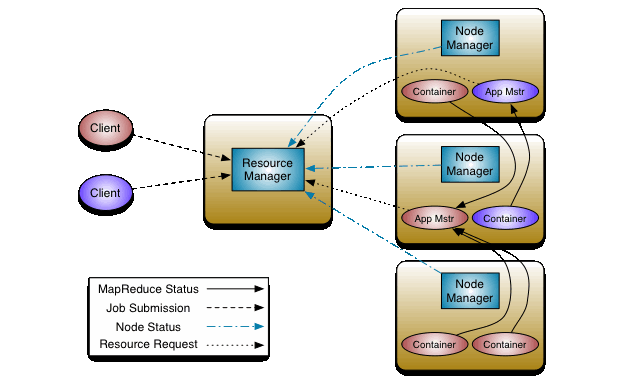
\includegraphics{./images/yarn_architecture.png}
    \caption[Architektur von YARN]
    {Architektur von YARN (entnommen aus \cite{HadoopYarnArch271})}
    \label{fig:yarnarch}
\end{figure}

Der \ac{RM} besteht aus zwei Kernkomponenten, dem \ac{AM} und dem \emph{Scheduler}.
Der \ac{AM} ist für die Annahme und Ausführung von einzelnen Anwendungen zuständig, denen der Scheduler die dafür notwendigen Ressourcen im Cluster zuteilt.

Der \ac{NM} eines jeden Nodes überwacht die Ressourcen seines jeweiligen Nodes sowie der auf dem Node ausgeführten Anwendungs"=Container und übermittelt diese dem \ac{RM}.

Jede YARN"=Anwendung bzw. Job besteht aus einer oder mehreren Ausführungsinstanzen, genannt \emph{Attempts}.
Die eigentliche Ausführung einer Anwendung findet in den bereits erwähnten \emph{Containern} statt, die jeweils einem Attempt zugeordnet sind.
Container können auf einem beliebigen Node ausgeführt werden und repräsentieren die Ausführung eines Tasks innerhalb der Anwendung.
Ein besonderer Container bildet hierbei der \ac{AppMstr}.
Er übernimmt das Monitoring der Anwendung und die Kommunikation mit dem \ac{RM} und \ac{NM} und stellt die dafür benötigten Informationen bereit \cite{HadoopYarnArch271}.
\todo{Evtl. noch ein paar Infos zur Node-Erkennung und zeitlichen abläufen}

Ein weiterer Bestandteil von Hadoop bzw. YARN ist der \ac{TLS}.
Er ist speziell dafür entwickelt, die Metadaten und Logs der YARN"=Anwendungen zu speichern und jederzeit, also als Anwendungshistorie, auszugeben \cite{HadoopYarnTlServer271}.

Das \textbf{\ac{HDFS}} basiert auf der gleichen Architektur wie YARN und besitzt ebenfalls einen Master und mehrere Slaves:

\begin{figure}[h]
    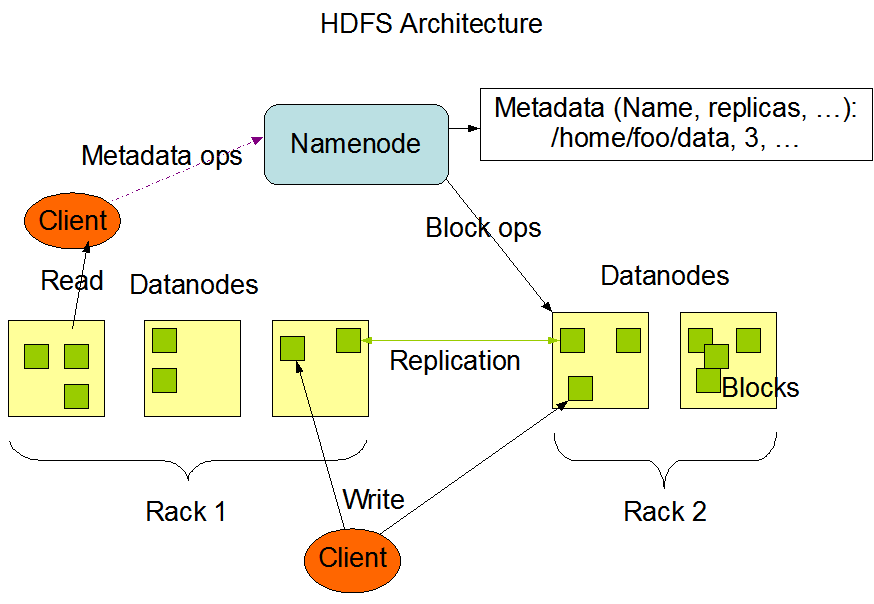
\includegraphics{./images/hdfsarchitecture.png}
    \caption[Architektur des HDFS]
    {Architektur des \acs{HDFS} (entnommen aus \cite{HadoopHdfsDesc271})}
    \label{fig:hdfsarch}
\end{figure}

Der \emph{NameNode} dient als Master für die Verwaltung des Dateisystems und reguliert den Zugriff auf die darauf gespeicherten Daten.
Unterstützt wird der NameNode vom \emph{Secondary NameNode}, der Teile der internen Datenverwaltung des \ac{HDFS} durchführt \cite{HadoopHdfsGuide271}].
Die Daten selbst werden in mehrere Blöcke aufgeteilt auf den \emph{DataNodes} gespeichert.
Um den Zugriff auf die Daten im Falle eines Node"=Ausfalls zu gewährleisten, wird jeder Block auf anderen Nodes repliziert.
Dateioperationen (wie Öffnen oder Schließen) werden direkt auf den DataNodes ausgeführt.
Sie sind darüber hinaus auch dafür verantwortlich, dass die gespeicherten Daten gelesen und beschrieben werden können \cite{HadoopHdfsDesc271}.

\textbf{MapReduce} bietet analog zu YARN die Möglichkeit, Anwendungen mit einem großen Ressourcenbedarf auf einem gesamten Cluster auszuführen.
Dazu werden bei einem MapReduce"=Job die Eingabedaten aufgeteilt, anschließend von den sog. \emph{Map Tasks} verarbeitet und deren Ausgaben von den sog. \emph{Reduce Tasks} geordnet.
\todo{Literatur für weitere Infos zu MR?}
Für die Ein- und Ausgabe der Daten wird in der Regel das \acs{HDFS}, für die Ausführung der einzelnen Tasks YARN genutzt \cite{HadoopMapRedTutorial271}.
Die MapReduce"=Komponente von Hadoop kann auch als Vorgänger von YARN angesehen werden, da YARN auch als \emph{MapReduce Next Gen} bzw. \emph{MRv2} bezeichnet wird und aufgrund der API"=Kompatibilität von YARN jede MapReduce"=Anwendung in der Regel auch auf YARN ausgeführt werden kann \cite{HadoopYarnArch271,HadoopYarnOverview271}.
